%\documentclass[12pt]{article}
%\usepackage[a4paper, margin=1in]{geometry} 
%\usepackage{graphicx} 
%\usepackage{hyperref}
%\usepackage{float}
%\usepackage{multicol}
%\usepackage{multirow}
%\usepackage{amsmath}
%\usepackage[font=small, labelfont=bf]{caption}
%
%\begin{document}

%
% Sequence profiles and patterns
%
\subsection{Sequence profiles and patterns}

%
% Protein secondary structures
%
\subsubsection*{Protein secondary structures}

\begin{figure}[H]
  \centering
      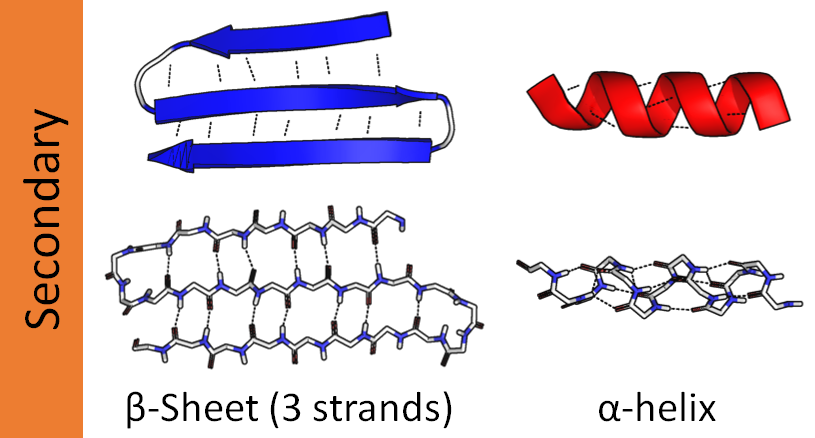
\includegraphics[width=0.5 \textwidth]{fig12/Alpha_beta_structure.png}
  \caption{Protein secondary structures (source: \href{https://commons.wikimedia.org/w/index.php?curid=56202452}{Shafee, Wikimedia Commons})}
\end{figure}

%
% Functional regions found in MSA
%
\subsubsection*{Functional regions found in MSA}

\begin{itemize}
\item \url{http://www.bioinformatics.org/strap/}
\item \url{http://journals.plos.org/plosone/article?id=10.1371/journal.pone.0070843}
\end{itemize}

%
% Applications of MSAs
%
\subsubsection*{Applications of MSAs}
\begin{itemize}
\item Position weight matrix
\item Sequence profile
\item HMM profile
\item Motifs
\end{itemize}

\bigskip 

%\end{document}
